%   % !TEX root = ../../VIII,3_Rahmen-TeX_9-0.tex
%  
%   Band VIII, 3 N.~?? 	(Unter)rubrik Auszüge
%
%   RK-Nr. 		58948
%	
%   Überschrift: 	(keine)
%   Titel: 			Aus und zu Huygens, Traité de la Lumière
%   Datierung:		Mitte September - 12 Oktober 1690
%
%   Diagramme: 		1
%
%
%
\selectlanguage{ngerman}
\frenchspacing
%
\begin{ledgroupsized}[r]{120mm}
\footnotesize
\pstart
\noindent\textbf{Überlieferung:}
\pend
\end{ledgroupsized}
%
\begin{ledgroupsized}[r]{114mm}
\footnotesize
\pstart \parindent -6mm
\makebox[6mm][l]{\textit{L}}%
Auszüge aus
\protect\index{Namensregister}{\textso{Huygens} (Hugenius, Ugenius, Hugens, Huguens), Christiaan 1629\textendash1695}%
C.~\textsc{Huygens}, %
\cite{00525}\textit{Traité de la lumière} \lbrack...\rbrack\ \textit{avec un discours de la cause de la pesanteur}, %
Leiden 1690, S.~14 und S.~173\textendash175:
%
LH~XXXV~11, 14~Bl.~33. 
Ein Zettel (ca.~6~x~4~cm.);
Ränder abgerissen;
geringfügiger Textverlust am unteren Rand von 33~v\textsuperscript{o}.
Zwei Seiten.
Auf Bl.~33~v\textsuperscript{o} tlw.\ Text ohne erkennbaren Zusammenhang mit dem Stück.
\pend
\end{ledgroupsized}
%
%
\count\Bfootins=1100%
\count\Afootins=1200%
\count\Cfootins=1100 
\vspace{5mm}
\begin{ledgroup}
\footnotesize
\pstart
\noindent%
\textbf{Datierungsgründe:}
Kurz nach der gemeinsamen Veröffentlichung von \cite{00525}\textit{Traité} und \textit{Discours}
%
verschickte \protect\index{Namensregister}{\textso{Huygens} (Hugenius, Ugenius, Hugens, Huguens), Christiaan 1629\textendash1695}C.~Huygens
%
am 8.\ Februar 1690 (\cite{01502}\textit{LSB} III, 4 N.~235, S.~460.15\textendash23) 
%
ein Exemplar des Bandes, das Leibniz erst im September zuging
%
(Erwähnung des Empfangs um den 12./22.\ September 1690: \cite{02066}\textit{LSB} III, 4 N.~274,
S.~559.22\textendash23).
%
%; N.~282: S.~598, Z.~14\textendash18; N.~283: S.~620, Z.~1\textendash2). 
%08./18.02. 1690 Huygens an Leibniz LSB III, 4 N. 235
%12./22.09.1690 an Bianchini LSB III,4 N. 274
%1.H. Oktober 1690 an Huygens LSB III, 4 N. 282
%03./13.10. 1690 an Huygens LSB III, 4 N. 283
%28.10./07.11.1690 an Huygens LSB III, 4 N. 287
%14./24.11.1690 an Huygens LSB III, 4 N. 292  
%
Die Abfassung der vorliegenden kurzen, notizhaften Auszüge, parallel zur ersten Lektüre der Werke, kann daher erst im September 1690 stattgefunden haben.
%
Dass dies außerdem kurz nach Empfang des Bandes geschah, geht aus den folgenden Umständen hervor.
%
\pend
%
\pstart
%
Leibniz exzerpiert auf Bl.~33~r\textsuperscript{o} aus dem \cite{00525}\textit{Traité de la lumière} eine Huygens'sche These über den mittelbaren Mehrkörperstoß. % Wird in RK41780 und RK58300 wieder aufgegriffen.
%
Zudem vergleicht er auf Bl.~33~v\textsuperscript{o} zwei Reihen. 
%
Es handelt sich um die Koeffizientenreihen der arithmetischen Hyperbel- und Kreisquadratur, die ebenfalls in 
%
der Publikation von 1690 besprochen werden:
%
In der \textit{Addition} zum \cite{00525}\textit{Discours de la cause de la pesanteur} (S.~173\textendash175)
%
präsentierte \protect\index{Namensregister}{\textso{Huygens} (Hugenius, Ugenius, Hugens, Huguens), Christiaan 1629\textendash1695}Huygens 
%
eine seines Erachtens neue Formel zur Quadratur der Hyperbel.
%
Nach eigenen Angaben hatte er seine Hyperbelreihe in Analogie zu Leibnizens bereits veröffentlichter arithmetischer Kreisquadratur 
%
(\cite{02042}\glqq De vera proportione circuli\grqq, \cite{01023}\textit{AE}, Februar 1682, S.~41\textendash46)
%
gebildet.
%
Leibniz hatte allerdings bereits in der Pariser Zeit die Quadraturfrage intensiv erforscht,
%
um 1673 die Kreisreihe (siehe \textit{LSB} VII,~6 \textit{passim}) 
%
und schließlich in verschiedenen ausführlichen Konzepten von 1676
%
eine allgemeine Kegelschnittreihe gefunden
%
(siehe \cite{01229}\glqq De quadratura arithmetica circuli ellipseos et hyperbolae\grqq, 
\textit{LSB} VII, 6 N.~51, bes.\ Prop.~XLIII, S.~618).
%
Er verzichtete auf eine Publikation der Konzepte, an deren Stelle er den viel kürzeren 
%
\cite{02042}Aufsatz von 1682 drucken ließ, bei dem das Augenmerk auf der Kreisquadratur lag.
%
Nach der Lektüre des \textit{Discours} reagierte Leibniz zügig, um einen Prioritätsanspruch über die Hyperbelquadratur zu erheben. 
%
In einem dahingehenden \cite{02045}Brief an 
%
\protect\index{Namensregister}{\textso{Mencke} (Menken, Menkenius, Menque), Otto 1644\textendash1707}Mencke
%
vom 2.\ (12.) Oktober 1690
%
(\cite{02045}\textit{LSB} III, 4 N.~281, bes.\ S.~588)
%
begründete er diesen Anspruch mit der Tatsache, dass die von 
%
\protect\index{Namensregister}{\textso{Huygens} (Hugenius, Ugenius, Hugens, Huguens), Christiaan 1629\textendash1695}Huygens 
%
veröffentlichte Formel zur arithmetischen Hyperbelquadratur
%
bereits aus seinen eigenen Publikationen hervorging: aus \cite{02042}\glqq De vera proportione circuli\grqq\ von 1682 in Verbindung mit
%
einigen Bemerkungen im \cite{01024}\glqq Schediasma de resistentia medii\grqq\ (\cite{01023}\textit{AE}, Januar 1689, hier S.~45).
%
Gleiches teilte er auch \protect\index{Namensregister}{\textso{Huygens} (Hugenius, Ugenius, Hugens, Huguens), Christiaan 1629\textendash1695}Huygens selbst
%
im \cite{01507}Brief vom 28.\ Oktober (7.\ November) 1690 (\textit{LSB} III, 4 N.~287, bes.\ S.~647.4\textendash16) mit.
%
Nachdem die \cite{01023}\title{Acta Eruditorum} im Oktober (S.~481\textendash487) und November (S.~561\textendash565) 1690
%
eine anonyme Besprechung
%
des Werkes gebracht hatten (\protect\vphantom)die wahrscheinlich von \protect\index{Namensregister}{\textso{Knorr} (Knorre), Martin 1657\textendash1699}M.~Knorre,
%
möglicherweise aber von 
%
\protect\index{Namensregister}{\textso{Tschirnhaus} (H.v.Tch., H.v.Tsch.), Ehrenfried Walther v. 1651\textendash1708}Tschirnhaus oder 
%
\protect\index{Namensregister}{\textso{Pfautz} (Pfauzius), Christoph 1645\textendash1711}Pfautz,
%
stammt; siehe \textit{LSB} III, 4, S.~586\protect\vphantom(),
%
entschied sich Leibniz zu einer öffentlichen Stellungnahme über die Priorität der Hyperbelquadratur.
%
Er verfasste mehrere Entwürfe für die \cite{01023}\textit{Acta Eruditorum}
%
und ließ schließlich diese und weitere Bemerkungen als 
%
\cite{02043}\glqq Additio ad Schediasma de medii resistentia\grqq\ drucken (\cite{01023}\textit{AE}, April 1691, S.~177f.), 
%
die er von einem eigens der \cite{02044}\glqq Quadratura arithmetica communis sectionum conicarum\grqq\ gewidmeten Aufsatz
%
begleiten ließ (\cite{01023}a.a.O., S.~178\textendash182).
%
\pend
\newpage
%
\pstart
Die vorliegenden kurzen Exzerpte stellen mit ihrem Notizcharakter wahrscheinlich das Zeugnis von
%
Leibnizens erster Berührung mit 
%
\protect\index{Namensregister}{\textso{Huygens} (Hugenius, Ugenius, Hugens, Huguens), Christiaan 1629\textendash1695}Huygens' 
%
Hyperbelreihe, somit auch die Grundlage für seine privaten und öffentlichen Äußerungen zur Prioritätsfrage 
%
ab dem 12.\ Oktober 1690, dar. 
%
Hieraus ergibt sich die vorgeschlagene Datierung von N.~\ref{58948}.
\pend 
\end{ledgroup}
%
%
\selectlanguage{latin}
\frenchspacing
% \newpage%
\vspace{8mm}
\pstart%
\normalsize%
\noindent%
%
\edtext{\lbrack33~r\textsuperscript{o}\rbrack\ Globi aequales\protect\index{Sachverzeichnis}{globi aequales}}{\lemma{\lbrack33~r\textsuperscript{o}\rbrack}\Bfootnote{\textit{(1)} Quatuor \textit{(2)} Globi \textit{(a)} quinque \textit{(b)} aequales \textit{L}}}
%
\textit{B}, \textit{A}, \textit{C}, \textit{C}, \textit{C}, etc. Globus\protect\index{Sachverzeichnis}{globus} \textit{A} tangit globos \edtext{plures\protect\index{Sachverzeichnis}{globus plures globos tangens}}{\lemma{}\Bfootnote{plures \textit{erg. L}}}
%
\textit{C}, \textit{C}, \edtext{\textit{C}. Quod si quiescat}{\lemma{\textit{C}.}\Bfootnote{\textit{(1)} Quod si ta \textit{(2)} Quod si quiescat \textit{L}}} 
%
\textit{A} \textit{C} \textit{C} \textit{C}, et \textit{A} feriatur a \edtext{\textit{B}. Manent}{\lemma{\textit{B}.}\Bfootnote{\textit{(1)} Transfert \textit{(2)} Manent \textit{L}}} 
%
immobiles \textit{B} et \textit{A} omnisque motus transfertur\protect\index{Sachverzeichnis}{translatio omnius motus} in globos\protect\index{Sachverzeichnis}{globus} \textit{C}, \textit{C}, \textit{C}, quotcunque sint. 
%
\edtext{Hugen.\protect\index{Namensregister}{\textso{Huygens} (Hugenius, Ugenius, Hugens, Huguens), Christiaan 1629\textendash1695} \textit{de lumine} c.~1.}%
{\lemma{Hugen.}\Cfootnote{%
\protect\index{Namensregister}{\textso{Huygens} (Hugenius, Ugenius, Hugens, Huguens), Christiaan 1629\textendash1695}\textsc{C.~Huygens},
\cite{00525}\textit{Traité de la lumière}, Leiden 1690,
chap.~1, bes. S.~14 mit Fig.\ 
(\textit{HO}\cite{00113} XIX, S.~459\textendash477, hier S.~473 mit Fig.~177).}} %
\pend
%
%
\vspace{2.0em} %%%%%%%%% Diagramm 1
\centerline{%
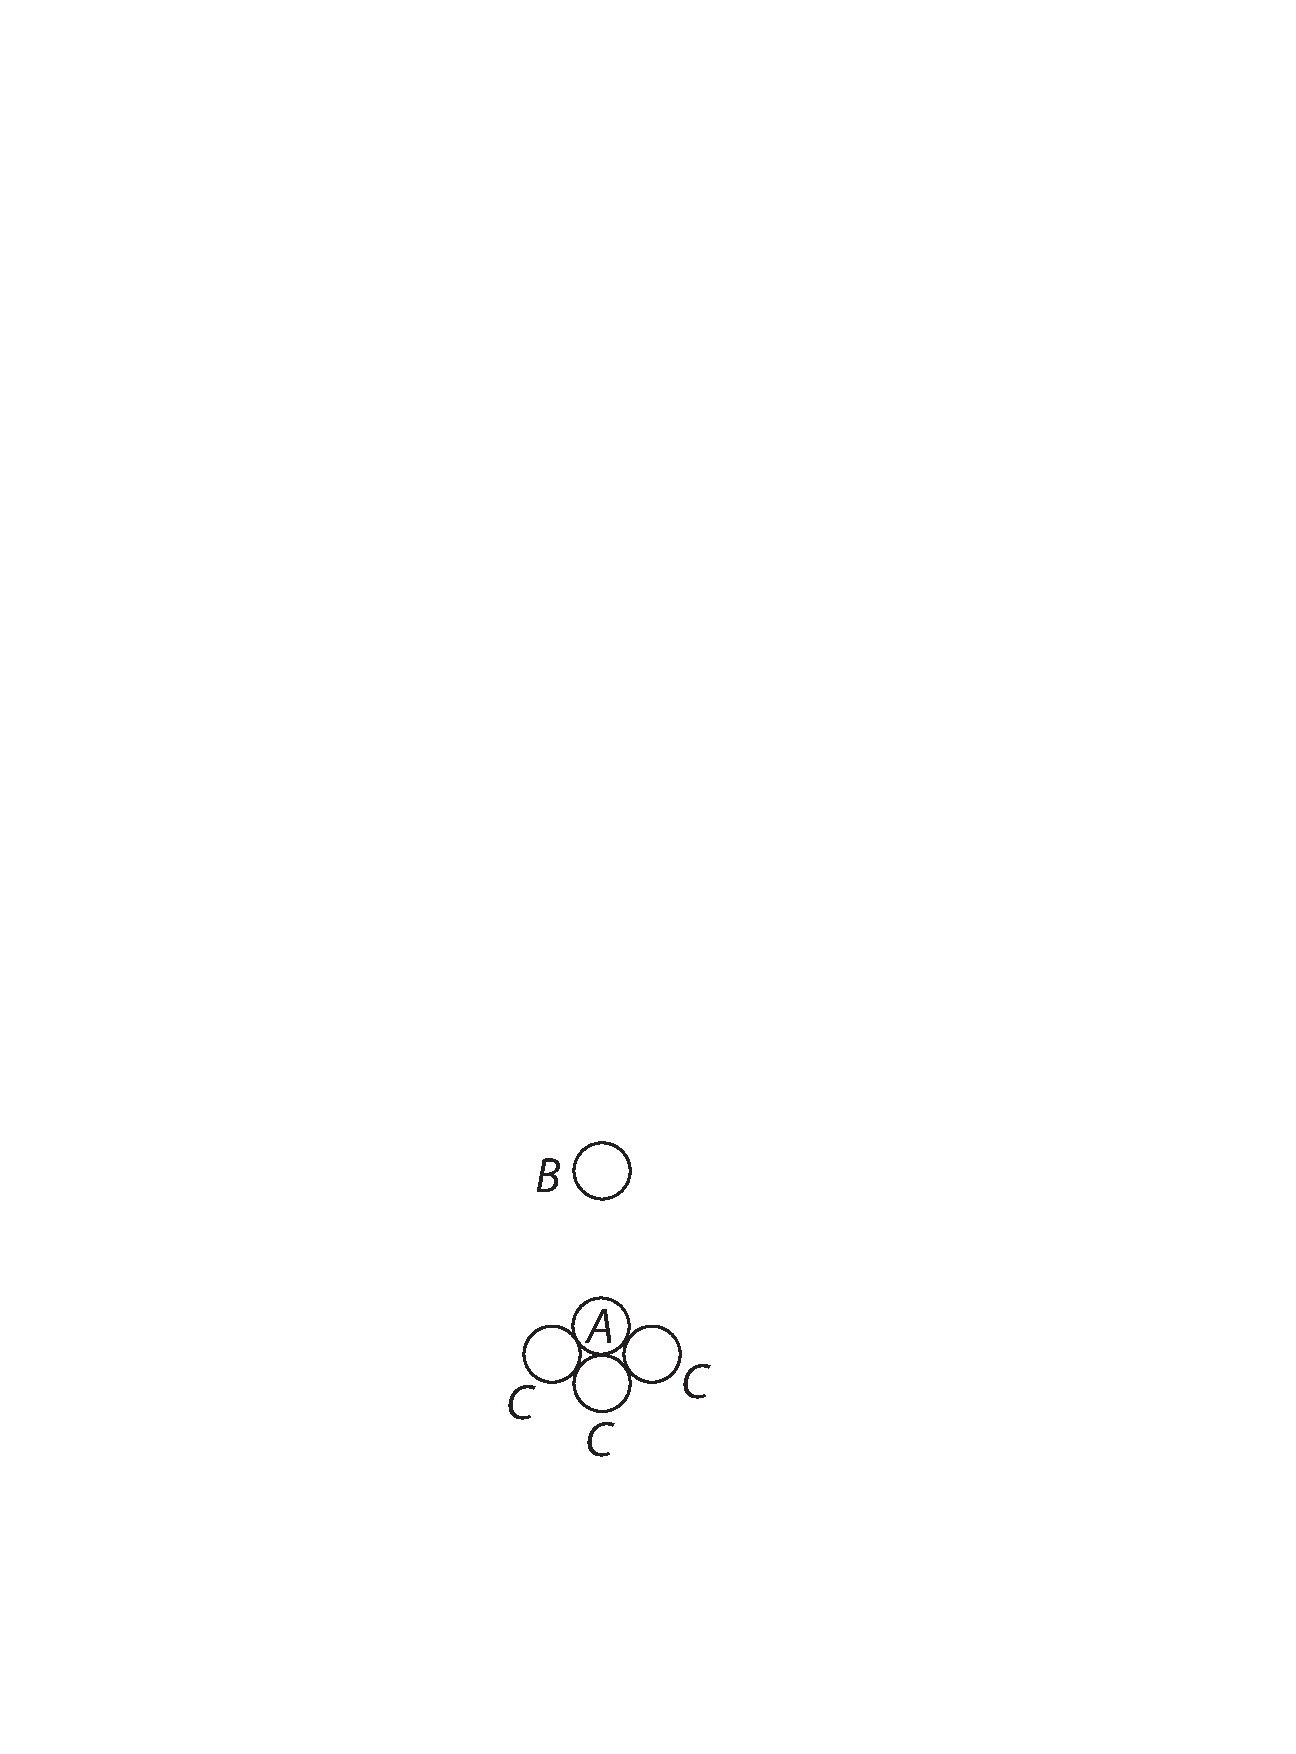
\includegraphics[width=0.13\textwidth]{%
gesamttex/edit_VIII,3/images/LH_35_11_14_033_d_033r.pdf%
}} 
\vspace{0.5em}
\centerline{%
\lbrack\textit{Fig.~1}\rbrack%
}
% \newpage%
\vspace{2.0em}
%
\pstart\noindent 
\lbrack33~v\textsuperscript{o}\rbrack\
%\pend
%
%\pstart
\lbrack\textit{Text ohne erkennbaren Zusammenhang mit dem Stück:}\rbrack
\pend
%
\vspace{0.5em} 
%
\pstart
\hfill
$\begin{array}{r}32\phantom{0} \\ 4\phantom{0} \\ \hline 128\phantom{0} \\ 2\phantom{0} \\ \hline 2560 \end{array}$
\hfill\hfill
$\displaystyle\efrac{\text{a e i o u}}{5}$
\hfill\hfill
\pend
%
\newpage
%
\pstart
\lbrack\textit{Senkrecht zur Schreibrichtung:}\rbrack
\pend
%
\vspace{1.0em} 
%
\pstart
\edtext{%
$\displaystyle\frac{\displaystyle\efrac{\displaystyle\frac{1}{1}+\displaystyle\frac{1}{3}+\displaystyle\frac{1}{5}+\displaystyle\frac{1}{7}+\displaystyle\frac{1}{9}}{1-\displaystyle\frac{1}{3}+\displaystyle\frac{1}{5}-\displaystyle\frac{1}{7}+\displaystyle\frac{1}{9\protect\vphantom{j}}}}{\phantom{.}1\hfill%
\phantom{iiii}\displaystyle\frac{\protect\vphantom{\sqrt1}1}{5}%
\phantom{ii}\hfill%
\Big\langle\displaystyle\frac{1}{9}\Big\rangle}$%
}{\lemma{$\displaystyle\frac{1}{1}+\displaystyle\frac{1}{3}+\displaystyle\frac{1}{5}+\displaystyle\frac{1}{7}+\displaystyle\frac{1}{9}$}%
\Cfootnote{%
Huygens stellt seine arithmetische Hyperbelquadratur ($a+\displaystyle\frac{1}{3}a^3+\displaystyle\frac{1}{5}a^5+\displaystyle\frac{1}{7}a^7+\displaystyle\frac{1}{9}a^9+\ldots$) im \cite{00525}\textit{Discours de la cause de la pesanteur}, S.~173\textendash175
(\textit{HO}\cite{00113} XXI, S.~482\textendash484), vor.}}%
\pend
\count\Bfootins=1200%
\count\Afootins=1200%
\count\Cfootins=1200 
%
%siehe **, S.~174 (HO **)
% Huygens 

%
